% Adapted for BMC Bioinformatics using the Springer Nature article template.
\documentclass[pdflatex,sn-vancouver-num]{sn-jnl}

\usepackage{graphicx}
\usepackage{amsmath,amssymb}
\usepackage{booktabs}
\usepackage{array}

\raggedbottom

\begin{document}

\title[DeepSeek pathology report understanding]{DeepSeek for pathology report understanding: strengths and limitations across extraction, staging, and prognosis tasks}

\author[1]{\fnm{Mohamed} \sur{Kone}}

\author*[1]{\fnm{Shulin} \sur{Wang}}\email{books@hnu.edu.cn}

\author[1]{\fnm{Gaoussou} \sur{Haidara}}

\affil*[1]{\orgdiv{School of Computer Science and Engineering}, \orgname{Hunan University}, \orgaddress{\city{Changsha}, \country{China}}}

\abstract{\textbf{Background:} Pathology reports contain clinically important information for cancer diagnosis, staging, and outcome research, but their unstructured format limits scalable reuse. We evaluated whether DeepSeek can support pathology report understanding across cancer type extraction, AJCC stage prediction, and prognosis classification.

\textbf{Methods:} We conducted an independent benchmark on PathRep-Bench style pathology report tasks derived from The Cancer Genome Atlas. The dataset contained 9,523 reports split into 7,618 training, 953 validation, and 952 test reports. DeepSeek V4 Flash and DeepSeek V4 Pro were evaluated using JSON-constrained prompting. Cancer type identification used non-reasoning prompting, whereas AJCC staging and prognosis prompting used reasoning-mode prompting. We also trained local TF-IDF logistic regression prognosis models and tested whether DeepSeek-extracted structured variables improved supervised prognosis modeling.

\textbf{Results:} DeepSeek V4 Flash achieved 0.9800 accuracy (95\% CI, 0.9695--0.9884) and 0.9778 macro F1 (95\% CI, 0.9660--0.9867) for cancer type identification. For AJCC stage prediction, DeepSeek V4 Flash achieved 0.8165 accuracy (95\% CI, 0.7845--0.8468) and 0.7841 macro F1 (95\% CI, 0.7421--0.8201) on 594 labeled test reports. DeepSeek V4 Pro did not significantly improve paired accuracy over Flash for either task and produced 14 empty final outputs during AJCC staging. DeepSeek prognosis prompting was weak on a 100-report subset, improving from 0.5083 to 0.5647 macro F1 with eight examples. A supervised TF-IDF text-only logistic regression classifier achieved the highest prognosis point estimate on the full test set, with 0.8571 accuracy and 0.8543 macro F1. Adding DeepSeek-extracted structured variables did not produce a statistically significant improvement.

\textbf{Conclusions:} DeepSeek is effective for pathology information extraction and provides strong AJCC staging support, but prognosis prediction is better framed as supervised outcome modeling under the evaluated framework. These findings support a hybrid architecture in which DeepSeek performs extraction and staging support, while supervised text-based models handle prognosis prediction.}

\keywords{pathology reports, large language models, DeepSeek, cancer staging, AJCC, prognosis, TCGA, natural language processing}

\maketitle

\section{Background}\label{sec:background}

Pathology reports are among the most information-rich documents in oncology. They summarize tumor histology, tissue site, grade, resection status, nodal involvement, metastatic findings, biomarker context, and in many cases explicit stage group. These reports are central to cancer diagnosis and treatment planning, but they are typically stored as free text. This makes large-scale reuse difficult for cohort construction, registry enrichment, outcomes research, and clinical trial screening.

Recent progress in large language models (LLMs) has made pathology report understanding more feasible. Unlike earlier rule-based systems or narrow named-entity recognition pipelines, LLMs can interpret varied report formats, follow label-constrained instructions, and produce structured outputs from heterogeneous text. PathRep-Bench established a useful benchmark for evaluating this capability across cancer type identification, AJCC stage identification, and prognosis assessment from pathology reports \cite{saluja2025pathrep,pathrepbench}. The benchmark highlights a natural difficulty gradient. Cancer type identification is often a direct extraction task. AJCC stage identification requires more reasoning over explicit stage statements, tumor extent, lymph nodes, and metastasis evidence. Prognosis prediction is still more difficult because it requires mapping report information to future clinical outcome.

Clinical NLP benchmarks such as BLUE and BLURB helped standardize evaluation across biomedical and clinical text tasks \cite{peng2019blue,gu2021pubmedbert}. Domain-pretrained models such as PubMedBERT and BioGPT showed the value of biomedical corpora for language-model pretraining \cite{gu2021pubmedbert,luo2022biogpt}. More recent biomedical LLM work has broadened from representation learning to instruction following, tool use, and clinical reasoning. Med-PaLM demonstrated that large instruction-tuned models can encode clinically useful knowledge for medical question answering \cite{singhal2023medpalm}. GeneGPT and related tool-augmented systems showed that LLMs can improve biomedical reasoning by calling domain resources instead of relying only on parametric knowledge \cite{jin2024genegpt}. GPTCelltype and other LLM-assisted biology workflows suggest that general-purpose LLMs can support expert annotation tasks, although such systems still require careful validation and task-specific evaluation \cite{hou2024gptcelltype}.

Pathology-specific LLM research has developed along two related tracks. One track focuses on pathology images and multimodal assistants, including foundation models and conversational systems for histopathology image interpretation \cite{lu2024pathchat}. Another track focuses on pathology report text, where the central problems are document understanding, label extraction, staging normalization, and outcome prediction. These report-understanding tasks are especially important because pathology text is already available at scale in many cancer datasets, but its free-text format makes direct computational reuse difficult.

DeepSeek is an attractive model family for this setting because it provides long-context API access, JSON output support, and low-cost inference options \cite{deepseekdocs,deepseekpricing}. However, its utility for pathology report understanding has not been independently characterized on the PathRep-Bench tasks. In particular, it is important to know whether a larger DeepSeek model improves performance enough to justify higher cost, and whether LLM-extracted variables add prognostic value beyond raw report text. This study evaluates DeepSeek across extraction, staging, and prognosis tasks using PathRep-Bench style TCGA pathology report splits. Our central hypothesis is that LLMs and supervised outcome models serve different roles: LLMs should excel at flexible information extraction and staging support, while prognosis prediction should benefit most from supervised learning directly optimized against outcome labels.

\section{Methods}\label{sec:methods}

\subsection{Dataset}\label{subsec:dataset}

We used the public PathRep-Bench data derived from TCGA pathology reports and TCGA clinical outcome resources \cite{pathrepbench,rosenthaldataset,liu2018tcga,weinstein2013tcga}. The prepared dataset contained 9,523 pathology reports with fixed train, validation, and test splits: 7,618 training reports, 953 validation reports, and 952 test reports. Each row included pathology report text, cancer type, AJCC stage fields where available, disease-specific survival time, and derived prognosis labels.

For cancer type identification, all 952 test reports had labels. For AJCC staging, 594 of the 952 test reports had usable high-level stage labels after excluding reports with missing stage labels. For prognosis, all 952 test reports had derived good or poor labels. The prognosis label was computed by cancer type: reports were labeled good if disease-specific survival time exceeded the cancer-type mean disease-specific survival threshold and poor otherwise. The mean threshold was estimated from the training split by cancer type, with fallback to all rows only if needed for a cancer type without training examples.

\subsection{Tasks}\label{subsec:tasks}

We evaluated three tasks. For cancer type identification, the model selected one label from 32 allowed TCGA cancer types. For AJCC stage identification, the model selected one of four high-level stage groups: Stage I, Stage II, Stage III, or Stage IV. The prompt instructed the model to map substages such as Stage IIA, Stage IIIB, or Stage IVA to the corresponding high-level stage group. For prognosis prediction, the model predicted good or poor prognosis from the pathology report text, cancer type, and cancer-type mean disease-specific survival threshold. This prognosis task was treated as a retrospective benchmark task and not as clinical advice.

\subsection{DeepSeek prompting framework}\label{subsec:deepseek}

All DeepSeek calls used JSON-constrained prompting through the chat completions API. The system instruction required valid JSON only, with no markdown or extra keys. The response format was set to JSON object mode. Cancer type identification used non-reasoning mode because the answer is usually directly stated in the report. AJCC staging and prognosis prompting used reasoning mode because these tasks require synthesizing stage evidence or outcome-relevant findings.

For cancer type identification, the prompt supplied the complete list of 32 allowed cancer type labels. For AJCC staging, the prompt supplied the four allowed high-level stage labels and instructed the model to use explicitly stated pathologic stage when available, map substages to their high-level group, and otherwise infer the best supported stage using tumor extent, nodal involvement, and distant metastasis evidence. For prognosis, the prompt supplied cancer type, the mean disease-specific survival threshold, and the pathology report. Zero-shot prognosis used no examples. Few-shot prognosis used eight training examples selected from the training split, balanced across good and poor labels.

\subsection{DeepSeek model comparison}\label{subsec:modelcomparison}

We compared DeepSeek V4 Flash and DeepSeek V4 Pro for cancer type identification and AJCC stage identification. For AJCC staging, both models were run with a 4,096 completion-token budget. Model output failures, including empty final responses and unparseable JSON, were counted as errors in the primary analysis.

\subsection{Prognosis machine-learning baselines}\label{subsec:ml}

We trained local logistic regression prognosis classifiers using the training and validation splits for training and the held-out test split for evaluation. The text-only model used TF-IDF features over pathology report text with lowercasing, English stop-word removal, unigrams and bigrams, sublinear term frequency, a minimum document frequency of 2, and a maximum of 50,000 features. Logistic regression used balanced class weights, the liblinear solver, C = 2.0, maximum 3,000 iterations, and a fixed random seed \cite{pedregosa2011scikit}.

We evaluated six prognosis feature sets: TF-IDF report text only; TF-IDF report text plus original structured fields; TF-IDF report text plus original structured fields plus DeepSeek-extracted variables; original structured fields plus DeepSeek-extracted variables without report text; DeepSeek-extracted variables only; and original structured fields only.

\subsection{DeepSeek-extracted variables for hybrid prognosis}\label{subsec:extraction}

To test whether LLM extraction could improve prognosis modeling, we used DeepSeek V4 Flash to extract structured variables from all training, validation, and test reports. The extraction schema included cancer type, AJCC stage, tumor size, positive nodes, examined nodes, distant metastasis, margin status, lymphovascular invasion, grade, necrosis, and key evidence phrases. Variable extraction used non-reasoning JSON prompting and was resumable. The final extraction covered 9,523 reports with 9 model-output errors. The extracted variables were converted into sparse dictionary features and added to the logistic regression prognosis pipeline.

\subsection{Cost and statistical analysis}\label{subsec:stats}

We estimated inference cost using recorded token usage from each run and DeepSeek pricing documentation \cite{deepseekpricing}. When cache-hit and cache-miss counts were unavailable, prompt tokens were conservatively priced as cache misses. We report estimated cost per report, cost per 1,000 reports, and cost per correct prediction.

We report accuracy and macro F1. Macro F1 was emphasized because prognosis labels were imbalanced and because staging performance can vary across classes. We estimated 95\% confidence intervals using nonparametric bootstrap resampling over reports with 2,000 bootstrap iterations and a fixed random seed. For paired model comparisons on the same reports, predictions were aligned by original row index. We used exact McNemar tests for paired accuracy comparisons and paired bootstrap differences for macro F1. Bootstrap comparison p values were computed as two-sided sign-crossing probabilities over the paired bootstrap distribution.

\section{Results}\label{sec:results}

\subsection{Cancer type identification}\label{subsec:cancerresults}

DeepSeek V4 Flash achieved near-ceiling performance for cancer type identification, correctly classifying 933 of 952 test reports. Accuracy was 0.9800 (95\% CI, 0.9695--0.9884) and macro F1 was 0.9778 (95\% CI, 0.9660--0.9867). There were no model-output errors (Table~\ref{tab:main}).

DeepSeek V4 Pro did not improve cancer type identification. It correctly classified 930 of 952 reports, with 0.9769 accuracy (95\% CI, 0.9664--0.9863) and 0.9685 macro F1 (95\% CI, 0.9394--0.9827). It also had no model-output errors, but its estimated cost was approximately 2.54 times higher than Flash for this task. The paired Flash-versus-Pro accuracy difference was not statistically significant by exact McNemar testing (6 Flash-only correct versus 3 Pro-only correct; p = 0.5078), and the macro F1 difference was not significant by paired bootstrap comparison (delta = 0.0094; 95\% CI, -0.0048 to 0.0363; p = 0.2330; Table~\ref{tab:paired}).

The main remaining cancer-type errors were clinically plausible neighboring-label errors, including rectum adenocarcinoma predicted as colon adenocarcinoma, stomach versus esophageal confusion, and renal cell carcinoma subtype confusion.

\subsection{AJCC stage identification}\label{subsec:stageresults}

DeepSeek V4 Flash achieved strong AJCC staging performance on the 594 test reports with stage labels. It correctly classified 485 reports, yielding 0.8165 accuracy (95\% CI, 0.7845--0.8468) and 0.7841 macro F1 (95\% CI, 0.7421--0.8201), with no model-output errors.

DeepSeek V4 Pro did not improve the primary AJCC stage result. It correctly classified 481 of 594 labeled reports, yielding 0.8098 accuracy (95\% CI, 0.7761--0.8401) and 0.6288 macro F1 (95\% CI, 0.5977--0.6573). The Pro run produced 14 empty final responses under the tested 4,096 completion-token budget. These empty outputs were counted as errors in the primary analysis. Among the 580 rows with valid JSON responses, Pro achieved 481 correct predictions, corresponding to 0.8293 accuracy; however, the empty-response reliability issue and higher cost made Flash the better primary model in this study. Flash did not significantly improve paired accuracy over Pro by McNemar testing (28 Flash-only correct versus 24 Pro-only correct; p = 0.6778), but it had significantly higher macro F1 in paired bootstrap analysis (delta = 0.1553; 95\% CI, 0.1234 to 0.1843; p $<$ 0.0001).

The largest AJCC error mode was under-calling Stage IV as Stage III. There were 24 Stage IV reports predicted as Stage III and 5 Stage III reports predicted as Stage IV. Adjacent-stage confusion also occurred among Stage I, Stage II, and Stage III.

\subsection{Prognosis prediction}\label{subsec:prognosisresults}

DeepSeek prognosis prompting was substantially weaker than extraction and staging. In a 100-report zero-shot run with DeepSeek V4 Flash, the model achieved 0.5300 accuracy (95\% CI, 0.4400--0.6300) and 0.5083 macro F1 (95\% CI, 0.4114--0.6033). An eight-shot prompt improved performance to 0.5700 accuracy (95\% CI, 0.4700--0.6700) and 0.5647 macro F1 (95\% CI, 0.4665--0.6599), but this remained far below the supervised prognosis models.

The strongest prognosis model was TF-IDF text-only logistic regression trained on the training plus validation splits and evaluated on the full 952-report test set. It achieved 0.8571 accuracy (95\% CI, 0.8351--0.8792) and 0.8543 macro F1 (95\% CI, 0.8312--0.8764). The model correctly classified 474 of 572 poor-prognosis cases and 342 of 380 good-prognosis cases.

Adding the original structured fields slightly reduced performance to 0.8529 accuracy and 0.8501 macro F1. Adding DeepSeek-extracted structured variables further reduced performance to 0.8435 accuracy (95\% CI, 0.8204--0.8666) and 0.8394 macro F1 (95\% CI, 0.8166--0.8630). DeepSeek variables without text were much weaker: original structured fields plus DeepSeek variables achieved 0.6512 macro F1, and DeepSeek variables alone achieved 0.6407 macro F1 (Table~\ref{tab:prognosis}).

Although the TF-IDF text-only model achieved the highest prognosis point estimate, adding DeepSeek-extracted variables did not produce a statistically significant improvement. The paired difference between TF-IDF text-only and TF-IDF plus structured fields plus DeepSeek variables was not statistically significant by exact McNemar testing (54 TF-IDF-only correct versus 41 DeepSeek-assisted correct; p = 0.2181) or paired bootstrap macro F1 comparison (delta = 0.0149; 95\% CI, -0.0047 to 0.0349; p = 0.1490). These results suggest that the raw pathology report text already captures much of the prognostic information available in this benchmark dataset under the evaluated modeling framework.

\subsection{Cost analysis}\label{subsec:costresults}

DeepSeek V4 Flash was consistently more cost-effective than DeepSeek V4 Pro in these experiments (Table~\ref{tab:cost}). For cancer type identification, Flash cost approximately USD 0.1918 per 1,000 reports, compared with USD 0.4871 per 1,000 reports for Pro. For AJCC staging, Flash cost approximately USD 0.2712 per 1,000 labeled reports, compared with USD 1.1717 per 1,000 labeled reports for Pro.

Full DeepSeek structured variable extraction across train, validation, and test reports cost approximately USD 1.77 for 9,523 reports. Although this extraction cost was low, the resulting variables did not improve prognosis performance over raw text.

\begin{table*}[htbp]
\caption{Main benchmark results with 95\% confidence intervals.}\label{tab:main}
\small
\begin{tabular}{@{}p{1.8cm}p{5.0cm}r p{3.0cm} p{3.0cm} r@{}}
\toprule
Task & Method & Rows & Accuracy (95\% CI) & Macro F1 (95\% CI) & Errors \\
\midrule
Cancer type & DeepSeek V4 Flash, JSON prompting & 952 & 0.9800 (0.9695--0.9884) & 0.9778 (0.9660--0.9867) & 0 \\
Cancer type & DeepSeek V4 Pro, JSON prompting & 952 & 0.9769 (0.9664--0.9863) & 0.9685 (0.9394--0.9827) & 0 \\
AJCC stage & DeepSeek V4 Flash, reasoning mode & 594 & 0.8165 (0.7845--0.8468) & 0.7841 (0.7421--0.8201) & 0 \\
AJCC stage & DeepSeek V4 Pro, reasoning mode & 594 & 0.8098 (0.7761--0.8401) & 0.6288 (0.5977--0.6573) & 14 \\
Prognosis & DeepSeek V4 Flash, zero-shot & 100 & 0.5300 (0.4400--0.6300) & 0.5083 (0.4114--0.6033) & 0 \\
Prognosis & DeepSeek V4 Flash, 8-shot & 100 & 0.5700 (0.4700--0.6700) & 0.5647 (0.4665--0.6599) & 0 \\
Prognosis & TF-IDF text-only logistic regression & 952 & 0.8571 (0.8351--0.8792) & 0.8543 (0.8312--0.8764) & NA \\
Prognosis & TF-IDF + structured fields + DeepSeek variables & 952 & 0.8435 (0.8204--0.8666) & 0.8394 (0.8166--0.8630) & NA \\
\botrule
\end{tabular}
\end{table*}

\begin{table*}[htbp]
\caption{DeepSeek cost analysis. Costs were estimated from recorded token usage and DeepSeek pricing.}\label{tab:cost}
\scriptsize
\begin{tabular}{@{}p{2.4cm}p{2.2cm}r r r r r r@{}}
\toprule
Run & Model & Reports & Correct & Tokens & Cost (USD) & Cost/report & Cost/1,000 \\
\midrule
Cancer type & V4 Flash & 952 & 933 & 1,292,828 & 0.182611 & 0.000192 & 0.1918 \\
Cancer type & V4 Pro & 952 & 930 & 1,294,297 & 0.463766 & 0.000487 & 0.4871 \\
AJCC stage & V4 Flash & 594 & 485 & 945,862 & 0.161103 & 0.000271 & 0.2712 \\
AJCC stage & V4 Pro & 594 & 481 & 1,170,725 & 0.695980 & 0.001172 & 1.1717 \\
Prognosis zero-shot & V4 Flash & 100 & 53 & 151,124 & 0.024516 & 0.000245 & 0.2452 \\
Prognosis 8-shot & V4 Flash & 100 & 57 & 386,105 & 0.058671 & 0.000587 & 0.5867 \\
\botrule
\end{tabular}
\end{table*}

\begin{table}[htbp]
\caption{Prognosis ablation results.}\label{tab:prognosis}
\small
\begin{tabular}{@{}p{7.0cm}r r r@{}}
\toprule
Prognosis model & Accuracy & Macro F1 & Delta \\
\midrule
TF-IDF text only & 0.8571 & 0.8543 & 0.0000 \\
TF-IDF text + original structured fields & 0.8529 & 0.8501 & -0.0042 \\
TF-IDF text + original structured fields + DeepSeek variables & 0.8435 & 0.8394 & -0.0149 \\
Original structured fields + DeepSeek variables & 0.6607 & 0.6512 & -0.2031 \\
DeepSeek variables only & 0.6492 & 0.6407 & -0.2136 \\
Original structured fields only & 0.5578 & 0.5540 & -0.3003 \\
\botrule
\end{tabular}
\end{table}

\begin{table*}[htbp]
\caption{Paired statistical comparisons. McNemar b/c indicates method A correct and method B wrong / method A wrong and method B correct. Positive deltas favor the first method in each comparison.}\label{tab:paired}
\small
\begin{tabular}{@{}p{4.8cm}r r p{1.5cm}r p{3.0cm}r@{}}
\toprule
Comparison & n & Delta acc. & b/c & McNemar p & Delta macro F1 (95\% CI) & Boot. p \\
\midrule
Cancer type: Flash vs Pro & 952 & 0.0032 & 6/3 & 0.5078 & 0.0094 (-0.0048 to 0.0363) & 0.2330 \\
AJCC stage: Flash vs Pro & 594 & 0.0067 & 28/24 & 0.6778 & 0.1553 (0.1234 to 0.1843) & $<$0.0001 \\
Prognosis: TF-IDF text-only vs DeepSeek-assisted ML & 952 & 0.0137 & 54/41 & 0.2181 & 0.0149 (-0.0047 to 0.0349) & 0.1490 \\
\botrule
\end{tabular}
\end{table*}

\begin{table}[htbp]
\caption{Selected clinically plausible error modes.}\label{tab:errors}
\small
\begin{tabular}{@{}p{3.4cm}p{3.7cm}p{3.7cm}r@{}}
\toprule
Error mode & Gold label & Predicted label & Count \\
\midrule
Rectum vs colon & Rectum adenocarcinoma & Colon adenocarcinoma & 5 \\
Kidney subtype & Kidney renal papillary cell carcinoma & Kidney renal clear cell carcinoma & 3 \\
Kidney subtype & Kidney renal clear cell carcinoma & Kidney chromophobe & 1 \\
Stage III/IV & Stage III & Stage IV & 5 \\
Stage III/IV & Stage IV & Stage III & 24 \\
\botrule
\end{tabular}
\end{table}

\begin{figure*}[htbp]
\centering
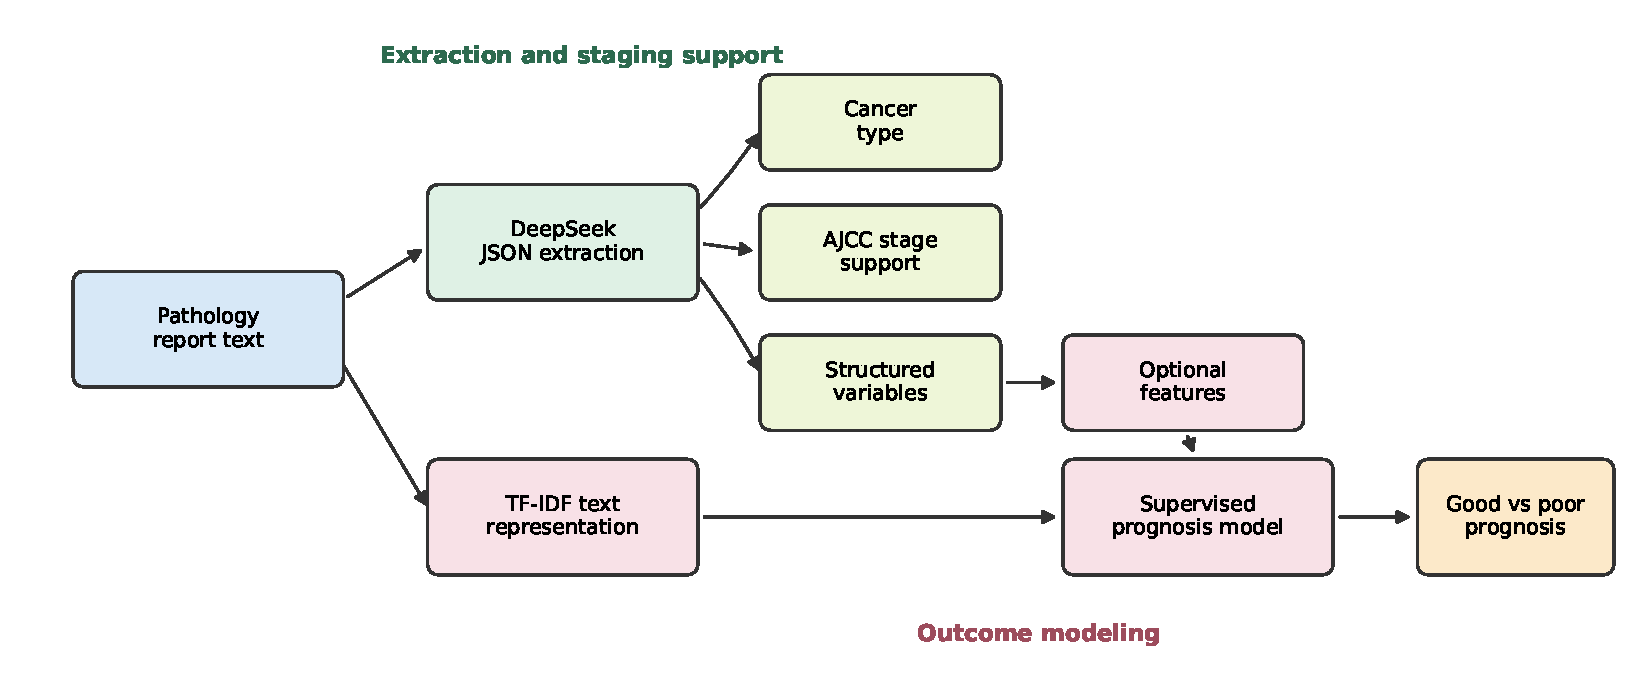
\includegraphics[width=\textwidth]{figures/hybrid_architecture.pdf}
\caption{Proposed role-separated architecture for pathology report understanding. DeepSeek is used for flexible language understanding tasks such as cancer type extraction, AJCC staging support, and structured variable extraction. Prognosis prediction is handled by a supervised outcome model trained directly against survival-derived labels, with raw report text retained as a primary representation.}
\label{fig:architecture}
\end{figure*}

\begin{figure*}[htbp]
\centering
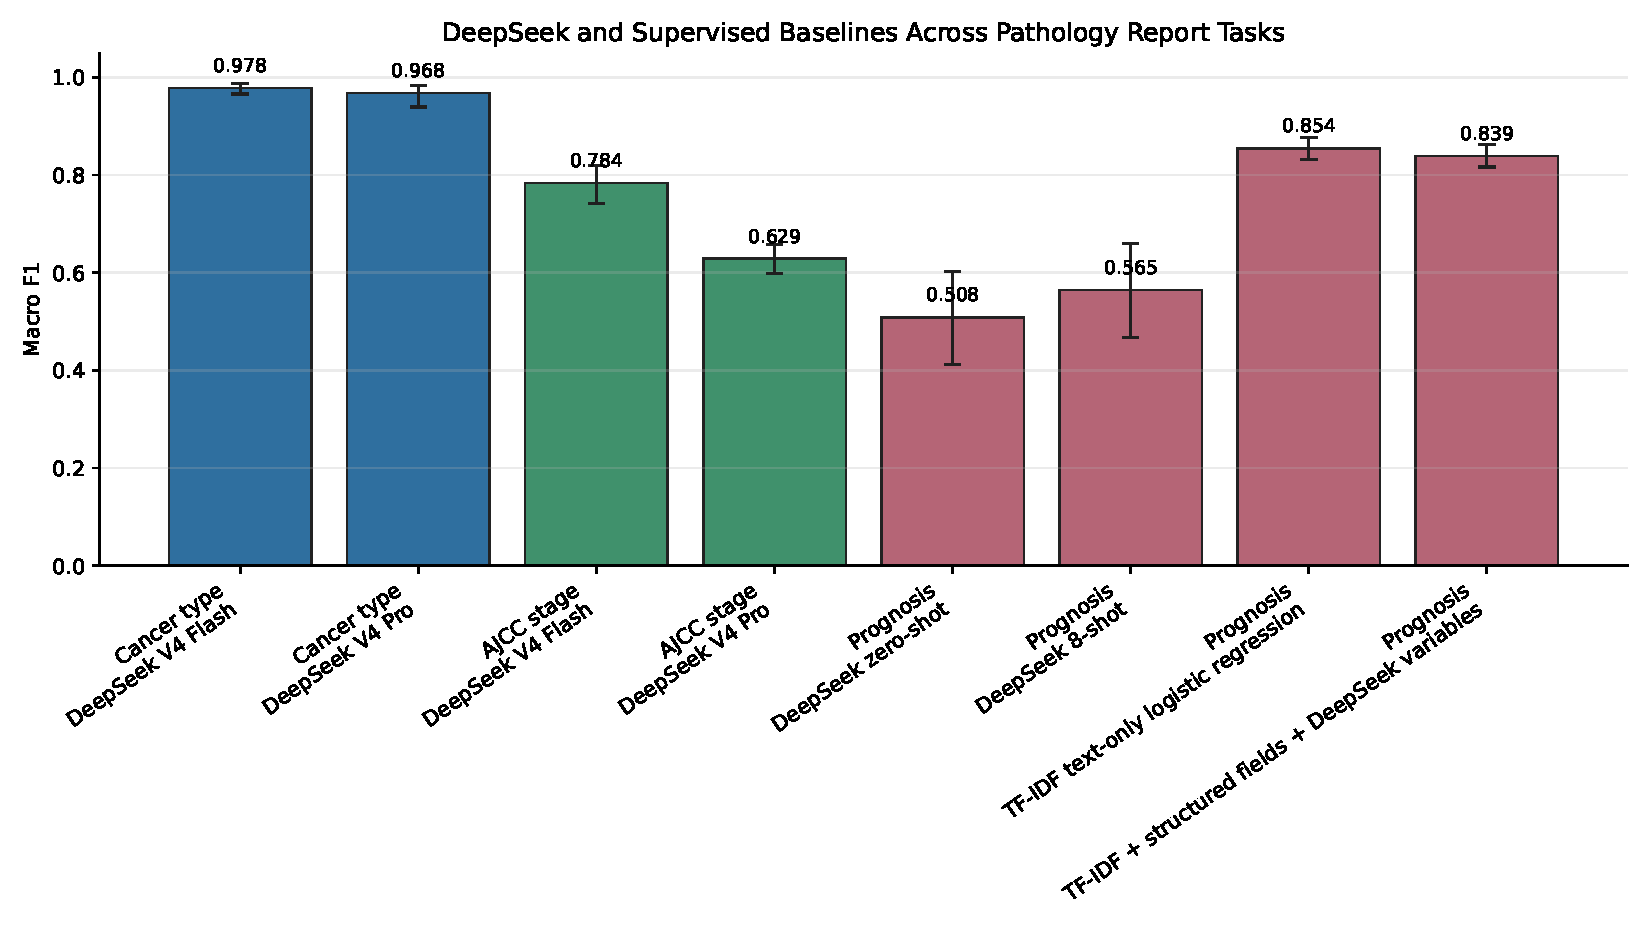
\includegraphics[width=\textwidth]{figures/macro_f1_results.pdf}
\caption{Macro F1 comparison across DeepSeek prompting conditions and supervised prognosis baselines. Error bars show 95\% nonparametric bootstrap confidence intervals over evaluated reports. Cancer type identification shows near-ceiling performance for both DeepSeek models, AJCC staging shows stronger Flash macro F1 under the tested completion budget, and prognosis performance is highest for supervised TF-IDF text modeling.}
\label{fig:macrof1}
\end{figure*}

\section{Discussion}\label{sec:discussion}

This study shows a clear role separation for DeepSeek in pathology report understanding. DeepSeek V4 Flash performed extremely well for cancer type identification and strongly for AJCC stage prediction. These are tasks where the desired answer is usually present in the report, although AJCC staging may require normalization from substage to high-level stage group or reasoning over tumor extent, nodal status, and metastasis information.

In contrast, prognosis prediction behaved differently. Prompting DeepSeek directly for good versus poor prognosis produced weak results on a 100-report subset, even after adding eight examples. More importantly, the full-test supervised ablation showed that the highest prognosis point estimate came from raw pathology report text represented with TF-IDF and modeled with logistic regression. Adding DeepSeek-extracted variables did not produce a statistically significant improvement over this text-only model, and DeepSeek-derived structured variables performed substantially worse when used without raw text.

This finding argues against treating LLM extraction as a universal improvement. LLMs can extract concise clinical variables, but prognosis prediction may depend on weak, distributed cues across the full report. These cues may include specimen context, wording around extent of disease, negative findings, tumor burden, procedure type, and co-occurring histologic details. Under the evaluated modeling framework, the raw report text appears to retain much of this prognostic information.

The Flash-versus-Pro comparison also has practical implications. DeepSeek V4 Pro did not improve cancer type identification and did not improve the primary AJCC staging result under the tested settings. For AJCC staging, Pro had slightly better valid-response accuracy after excluding empty outputs, but this was offset by 14 empty final responses and substantially higher cost. These results suggest that, for structured pathology extraction and staging support, a cheaper fast model may offer the better cost-performance tradeoff.

The error analysis supports the interpretation that DeepSeek failures are often clinically plausible rather than random. For cancer type identification, the most prominent pattern was rectum adenocarcinoma predicted as colon adenocarcinoma (Table~\ref{tab:errors}). Kidney cancer subtype errors were also observed, particularly papillary renal cell carcinoma predicted as clear cell carcinoma. For AJCC staging, the most important error mode was Stage IV under-called as Stage III. In some pathology reports, metastatic information may be absent, historical, or described outside the main specimen diagnosis, making this distinction difficult from pathology text alone.

The results support a hybrid architecture (Figure~\ref{fig:architecture}). DeepSeek should be used where flexible language interpretation is valuable: cancer type extraction, staging support, conversion of reports into structured variables, and possibly evidence highlighting for review. Prognosis prediction should be treated as supervised outcome modeling, preferably using raw report text and, in future work, survival-analysis methods that account for censoring and time-to-event structure.

\section{Limitations}\label{sec:limitations}

This study has several limitations. First, it is retrospective and based on public TCGA-derived pathology report data. Performance may differ for contemporary institutional reports, scanned reports, synoptic templates, or reports with different cancer-type distributions. Second, the prognosis label is a simplified binary endpoint derived from cancer-type mean disease-specific survival. This does not replace formal survival modeling and does not account for censoring in the way a Cox model, random survival forest, or other time-to-event method would.

Third, DeepSeek prognosis prompting was evaluated on a 100-report subset rather than the full test set. The subset result is sufficient to show that direct prompting was weak in the tested setting, but full-set prompting would be needed for a definitive LLM-only prognosis leaderboard. Fourth, AJCC staging from pathology reports alone is inherently limited. Some stage-defining information, particularly distant metastasis and clinical staging context, may not be present in pathology text. A clinically deployed staging support system should combine pathology text with structured clinical data, radiology, operative notes, and registry fields.

Fifth, DeepSeek V4 Pro was evaluated with a 4,096 completion-token budget for AJCC staging. The 14 empty final responses suggest that a larger completion budget or different reasoning configuration might improve reliability. The primary conclusion is therefore cost-performance under the tested settings, not an absolute statement about the maximum achievable performance of Pro. Finally, confidence intervals and paired tests were based on bootstrap resampling and exact McNemar tests over the available benchmark rows. These analyses quantify uncertainty in the current test set but do not replace external validation on independent institutional cohorts.

\section{Conclusions}\label{sec:conclusions}

DeepSeek V4 Flash is a strong and cost-effective model for pathology report understanding. It achieved near-ceiling cancer type identification and strong AJCC staging performance using JSON-constrained prompting. DeepSeek V4 Pro did not improve performance enough to justify its higher cost in the tested settings.

Prognosis prediction remained the main limitation. Direct DeepSeek prompting was weak, and DeepSeek-extracted structured variables did not significantly improve a supervised prognosis model beyond a simple TF-IDF representation of raw report text. This suggests that prognosis is better framed as supervised outcome modeling rather than pure LLM prompting or LLM extraction under the evaluated benchmark framework.

\backmatter

\bmhead{Supplementary information}

Not applicable.

\bmhead{Acknowledgements}

Not applicable.

\section*{Declarations}

\bmhead{Funding}

The authors received no specific funding for this work.

\bmhead{Competing interests}

The authors declare that they have no competing interests.

\bmhead{Ethics approval and consent to participate}

This study used public, de-identified TCGA-derived pathology report benchmark data. No new human participant data were collected for this study.

\bmhead{Consent for publication}

Not applicable.

\bmhead{Availability of data and materials}

The public benchmark data are available from the PathRep-Bench project repository and TCGA pathology report resources \cite{pathrepbench,rosenthaldataset}. The adapted DeepSeek benchmarking code and derived non-sensitive manuscript outputs are available at \url{https://github.com/mohkone/DeepSeekPathrep}. A Zenodo archive DOI should be added after repository archiving and before journal submission.

\bmhead{Code availability}

The analysis code is available at \url{https://github.com/mohkone/DeepSeekPathrep}. A Zenodo archive DOI should be added after repository archiving and before journal submission.

\bmhead{Authors' contributions}

MK conducted the computational experiments, analyzed the results, and drafted the manuscript. SW supervised the study, contributed to the study design, and revised the manuscript. GH contributed to interpretation of results and manuscript review. All authors read and approved the final manuscript.

\bibliography{deepseek_pathrep_bmc}

\end{document}
